\section{HEADS: A Generative Middleware Approach for the Development of HD Services}

Rather than providing yet another programming language supposedly able to address all the concerns needed for HD services, the HEADS approach proposes to rely on abstractions on top of existing programming languages to: 
\begin{itemize}
\item enable the integration of existing C/C++, Java, JavaScript libraries (and potentially libraries in other languages). In other words, promoting an existing library as a HEADS component, which can then be manipulated by the different tools provided by HEADS, should only require a minimal effort. 
\item provide expressive constructs to implement the necessary "glue code" to ensure that different libraries (potentially in different languages) can communicate locally or asynchronously over a network 
\item ease the reuse of fragments of logic across different platforms and languages 
\item ease the deployment, operation and maintenance of large-scale and distributed assemblies of heterogeneous component.
\end{itemize}

HEADS also intensively rely on generative techniques to produce C/C++, Java, JavaScript code, which: 
\begin{itemize}
	\item aims at being as efficient and as readable as code written by experienced programmers. In particular, the generated code is idiomatic e.g. proper Object-Oriented Java code for the JVM versus optimized C code with no dynamic allocation for small micro-controllers. 
\item provides clear public APIs to enable any programmer to interact with it with no need for her to use any HEADS-specific tool, just her favorite C/C++, Java, JavaScript editor or IDE. 
\item has few (ideally none) dependencies to any HEADS runtime libraries
\end{itemize}

The HEADS Design Language and Transformation Framework are available as an open-source projects on GitHub\footnote{https://github.com/SINTEF-9012/ThingML}.

\subsection{HEADS Design Language}

The ambition of the HEADS design language is to support the implementation and integration of the different parts of HD-services, including the integration of legacy and of-the-shelf components and libraries. The HEADS approach has a cost that comes as a consequence of this flexibility. At a certain abstraction level, all components interfaces need to be described in terms of the HEADS modeling language in order to allow for their integration in the system. However, it is important for any existing platform, library, framework or middleware to be usable without re-inventing, re-modeling or re-implementing it. In the design of the HEADS approach and code generation framework, a special attention is put to avoid introducing any accidental overhead beyond what is strictly necessary for the integration of the implementation artifacts. 

For the components developed from scratch or for which the target runtime environment might change, the HEADS design language provides with all the required expressiveness to fully specify the behavior of a component in a platform independent way. Different code generators can then be used to produce code for different platforms (currently Java, JavaScript and C/C++). This is similar to typical Model-Driven Engineering platform-independent models with a set of code generators (or compilers) for different platforms. At the other end of the spectrum, for the integration of an existing component, the HEADS approach allow modeling only the required part of interface of the component and mapping to its public platform specific API. 

This is similar to typical wrapping of external components and libraries such as for example Java Native Interface for Java to interact with a native library. The contribution of the HEADS approach is to give the flexibility to develop components which are neither fully platform independent nor direct wrapping around existing components but rather an arbitrary combination of existing libraries, platform features and application logic. In practice most of the components of a HD-service fall under this category and efficiently being able to integrate these different elements a key goal. The way the HEADS approach implements such capabilities is two-fold. First, a set of special constructs and actions are included in the HEADS action languages in order to seamlessly interleave platforms specific code and platform independent code. Second, the HEADS approach relies on a highly customizable code generation framework which can be tailored to specific target languages, middleware, operating systems, libraries and even build systems, as described in the next sub-section.

\subsubsection{Defining the interfaces of components}

The HEADS Design Language provides constructs to implement lightweight components which communicate asynchronously with other components. In the case of a distributed system running on top of a heterogeneous infrastructure, stronger assumptions regarding communication are simply not realistic. The API of a component basically follows a format well-established in the CBSE community: a set or ports specifying which message can be sent and received by the component. 

For example, a timer component would describe the following API: 

%\begin{ls}

\begin{lstlisting}
thing fragment TimerMsgs {  
  message start(delay : Integer); // Start the Timer 
  message cancel(); // Cancel the Timer  
  message timeout(); // Notification 
} 
thing fragment Timer includes TimerMsgs {  
  provided port timer {  
    sends timeout  
    receives start, cancel 
  } 
}
\end{lstlisting}


Note that ports are bi-directional as they can both send and receive message. Our notion of port should be understood as an atomic service, which is either provided or required. The service itself typically requires exchanging a set of message, typically a request (like \texttt{start}) and a response (like \texttt{timeout}). 

\subsubsection{Wrapping existing libraries}
A timer component is typically useful in any language. The API we have just defined in fully platform-independent, as it contains no Java, JavaScript or C/C++. As all those languages already providing native timing facilities, we simply need to wrap those facilities into platform-specific components.  

The script below shows how the timer is implemented in JavaScript, simply by relying on JavaScript timers: 

\begin{lstlisting}
thing TimerJS includes Timer {  
  function cancel() do 'clearTimeout(this.timer);' end  
  function start(delay : Integer) do  
    'this.timer = setTimeout(function(){' 
    timer!timeout()  
    '},' & delay & ');'  
  end  
  statechart SoftTimer init default {  
    state default {  
      internal start event m : timer?start  
      guard m.delay > 0  
      action start(m.delay)  
      internal cancel event m : timer?cancel  
      action cancel()  
    }  
  }  
} 
\end{lstlisting}

Basically, anytime a start message is received on the timer port, we first check that the delay is positive. If so, we call the start function, which is a simple wrapper around the native \texttt{setTimeout} function provided in JavaScript. Native code {\em i.e.} code that is directly expressed in the target language (here JavaScript) should be written between simple quotes. Native code can be interleaved with actions and expression of the HEADS Modeling Language. This way, the developer does not need to know how the generated code will look like to be able to wrap her library. No matter if the delay variable is renamed in the generated e.g. to avoid name conflict or if the action of sending the timeout actually implemented in a generated function called \texttt{sendtimeoutOnTimer}. She just can simply refer to the delay variable and send a message with no knowledge of the underlying implementation of those mechanisms. 

In the same way, the timer can be mapped to Java:

\begin{lstlisting}
object JThread @java_type "Thread" 
property timer : JThread 

function start(delay : Integer) do  
  timer = 'new Thread() { 
    public void run() { 
    sleep(' & delay & ');' 
    timer!timer_timeout() 
  '};' 
  '' & timer & '.start();' 
end 
\end{lstlisting} 

\subsubsection{Implementing components}

To orchestrate messages and define the behavior of components, beyond the wrapping of existing libraries of components, the HEADS Design Language provides a set of facilities: 
\begin{itemize}
\item Imperative programming to implement simple procedures, either directly using the actions and expression languages provided by the HEADS Modeling Language or by using the features of the target languages (or a mix of both) 
\item Event-Condition-Action (ECA) rules, which basically allows reacting to incoming events, independently from any state e.g. unconditionally shut down the system if emergency button has been pressed.  
\item Composite State Machine, also including parallel regions, which allows reacting to a sequence of incoming events e.g. to make sure all drivers are initialized in the proper order before accepting any other command 
\item Complex Event Processing (CEP), which allows reacting to patterns in large flows of events, without explicitly defining all possible sequences of events.
	\end{itemize}

The combination of those four paradigms enables service developers to express advanced behavior, which can efficiently tame large flows and data and process them to infer relevant information, as illustrated in Figure~\ref{fig:fig1}. A typical use-case is to use imperative programming to write drivers interacting with the physical world (sensors, actuators) or 3rd party software systems. As existing programmatic imperative APIs already exist, they can easily be integrated with the imperative approach. 

\begin{figure}[h]
\centering
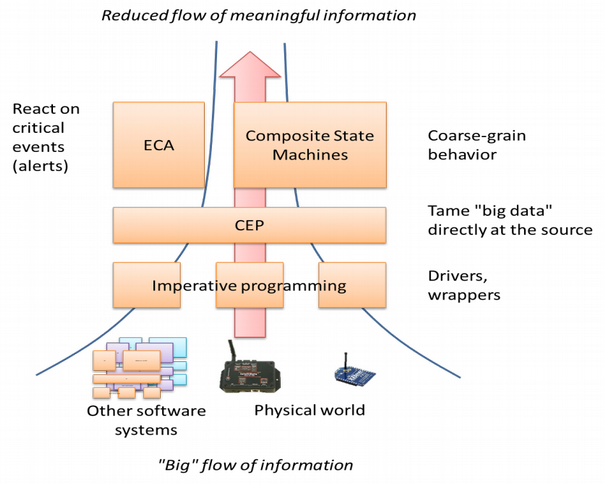
\includegraphics[width=0.7\linewidth]{figures/fig1}
\caption[Event Processing]{Event Processing}
\label{fig:fig1}
\end{figure}


As sensors might generate a large amount of data, a CEP layer close to the sensors enables service designers to express rules able to handle those data and to extract some relevant information (e.g. alert, status). The ECA paradigm is then particularly suited to handle alerts as they enable to enact some reflex-like actions (similarly to the way the spine "shortcuts" the brain to enact a fast movement e.g., when one burns his finger). Finally, composite state machines enable to describe advanced behavior, orchestrating and adapting to a set of events coming from the CEP. 

The HEADS Design Language is conceptually a usable sub-set of the UML (Composite Statecharts and Component Diagrams) with a syntactical notation rather than a graphical notation, so that it remains closer what programmers already know. In addition to the introduction of CEP in state machines, a key difference with UML is that our language comes with a first class action language so that models are not polluted with so-called "Opaque Behavior" (basically a String where code from the target language is directly outputted). This action language is basically the common subset of what is found in most languages, including numerical and Boolean algebra, control structures, functions, variable declaration and assignments, etc. The only action that is not typically found in programming language is the ability to asynchronously send a message through a port (rather than a simple method call). 

ECA rules are basically internal transitions, as in the JavaScript timer. Those rules basically react on an event and can be optionally guarded with any boolean expression, e.g. involving properties of the component and/or parameters of the message. Any action can then be triggered, either fully expressed at a platform-independent level or mixed with the target language (as in the JavaScript timer). As for the state machine, we support all the concepts present in the UML, including composite states and concurrent regions.  

The CEP concepts currently included in the HEADS Modeling Language is a sub-set of the concepts of ReactiveX (or other CEP language such a EPL available in Esper). We provide support for joining and merging flows of events, time or length windows and arbitrary filters.  

\begin{lstlisting}
stream lengthW 
  from e : [weather1?temp | weather2?temp]::keep if inRange(e)::during 1000*60 by 1000*60
  select avg : average(e.t[]),  
         min : min(e.t[]),  
         max : max(e.t[])  
action report!temp(avg, min, max)
\end{lstlisting}

This CEP stream illustrate most of the concepts currently integrated. It performs a merge between two temperature sensors (connected on ports weather1 and weather2). Basically, all temperature measurements coming from both sensor will be piped in a new stream. All these measurements are then filtered using a custom \texttt{inRange} operator defined by the developer, which will discard values that are outside a range and which are most likely due to an erroneous measurement rather than a correct measurement being too cold or too warn. The merging and the filtering happens on a time window during one minute which progress by slices of one minute. While such kind of CEP query could be implemented directly in Java, JavaScript or C, or at a more abstract level using the HEADS Modeling Language (state machine), it alleviates in any case the developer from writing a lot of "plumbing code" (timers, buffers, etc), which if not implemented correctly can have dramatic impact on memory and performances.

\subsection{HEADS Transformation Framework}

The HEADS Transformation Framework is responsible for ``compiling''  HEADS Design Models into source code for a large variety of languages. Rather than implementing one monolithic compiler for each language we target, the HEADS Transformation Framework instead is architected as a modular object-oriented framework. This framework promotes reuse of code among different compilers. A total of 8 formal extension points have been identified in the HEADS code generation framework in order to allow the developer to easily and efficiently customizing some parts of the code generation while reusing the rest. 

\subsubsection{Role of the extension points}

\paragraph{Actions / Expressions / Functions }


The implementation of this extension point consists of a visitor on the Actions and Expressions part of the HEADS Design Language. New code generators can be created by inheriting from that abstract visitor and implementing all its methods. Alternatively, if only a minor modification of an existing code generator is needed, it is possible to inherit from the existing visitor and only override a subset of its methods. Most of the actions and expressions (26 out of 35 concepts) is actually defined in the framework, as most of the programming languages have similar syntax for numerical and Boolean algebra, control structures, etc. The script below shows how a if  condition with optional else is compiled. The same code is reused in all Java, JavaScript and C compilers. 

\begin{lstlisting}[language=Java]
@Override 
public void generate(ConditionalAction action, StringBuilder builder, Context ctx) { 
  builder.append("if("); 
  generate(action.getCondition(), builder, ctx); 
  builder.append(") {\n"); 
  generate(action.getAction(), builder, ctx); 
  builder.append("\n}"); 
  if (action.getElseAction() != null) { 
    builder.append(" else {\n"); 
    generate(action.getElseAction(), builder, ctx); 
    builder.append("\n}"); 
  } 
  builder.append("\n"); 
} 
\end{lstlisting}

\paragraph{Behavior implementation}
This part of the code generator corresponds to the code generated from the state machine structures, ECA and CEP rules contained in Things. There is basically two main strategies to compile the behavior: target frameworks that are able to execute state machines and CEP or generate the whole logic to keep full control of what is executing at runtime. The first option is typically chosen for high-level languages not intended to run on resource-constrained devices, as it simplifies the code generation process (less code to generate) and generally improve the readability and maintainability of the generated code (less code to read and maintain). On resource-constrained devices however (down to 2 KB RAM) it is of primary importance to have control of every byte allocated and the overhead of embedding a framework is usually to heavy. The HEADS Transformation Framework does not impose nor favors any of those approaches and both can be implemented. The Java and JavaScript compilers use a framework approach whereas the family of C compilers use a full generative approach. In both cases, the framework provides support in the form of a set of helpers which pre-process the state machine e.g. to provide the list of all outgoing transitions for a given state, or the list of all messages being actually used by a component. 

\paragraph{Ports / Messages /APIs}

This part of the code generator corresponds to the wrapping of the generated code into reusable components on the target platform. Depending on the target platform, the language and the context in which the application is deployed, the code generated can be tailored to generate either custom modules or to fit particular coding constraints or middleware to be used on the target platform. As a best practice, the generated modules and APIs for things should be manually usable in case the rest of the system (or part of it) is written directly in the target language. For example, in object oriented languages, a facade and the observer pattern can be used to provide an easy to use API for the generated code. In C, a module with the proper header with structures and call-backs should be generated. 


The following code for example generates a Java interfaces that any Java programmer can use to send messages to a generated component. 

\begin{lstlisting}[language=Java]
for (Port p : thing.allPorts()) { 
  StringBuilder builder = ctx.getNewBuilder(thing.getName() + "_" + p.getName() + ".java"); 
  builder.append("public interface " + "I" +  
  thing.getName() + "_" + p.getName() + "{\n"); 
  for (Message m : p.getReceives()) { 
    builder.append("void " + m.getName() + "_via_" + p.getName() + "("); 
    generateParameter(m, builder, ctx); 
    builder.append(");\n"); 
  } 
  builder.append("}"); 
}
\end{lstlisting}

For example, for the Java timer component, this would generate this simple API: 


\begin{lstlisting}
public interface ITimerJava_timer{ 
	void start_via_timer(short delay); 
	void cancel_via_timer(); 
}
\end{lstlisting}

\paragraph{Main and Build}

These two extension points are responsible for providing users with a turn-key solution to compile and run the generated code. In the main file, all components and instantiated and connected. The build files automate all tasks needed to properly compile e.g. fetching dependency. For the users, compiling and running the code is as simple as: 

\begin{lstlisting}[language=bash]
mvn install exec:java #for Java 
npm install && node main.js #for JavaScript
make && ./myProgram #for C 
\end{lstlisting}

This extension point makes it easy to for example switch from Maven to Gradle for the build of Java project. 

\paragraph{Message Queing, Scheduling and Dispatching}

Those extension points are related to the internal management of messages within a node. By default, messages are queued in a FIFO, typically reusing already structures. On some very constrained platforms (microcontrollers) the code for the FIFO also needs to be generated as the standard library is typically more limited.For the scheduling and dispatching of messages we typically rely on facilities available on the OS (threads) to ensure a fair distribution of messages among components and avoid starvation and race conditions. Again, on very constrained platforms that are too limited to run an OS, custom schedulers should be generated.

\paragraph{Connectors}

This extension point is concerned with the serialization and transport of messages among components distributed over the network. For the serialization a default serialization of messages into arrays of bytes is provided~\cite{DBLP:conf/models/FleureyMSB11}, but developers can implement their own serialization. For example, we are currently implementing a generator to integrate with MessagePack~\cite{furuhashimessagepack}. For the transport itself, we usually rely on the large collections of communication channels already available in the HEADS Runtime platform (see next section): MQTT, WebSocket, Serial, etc. 

\subsubsection{Benefits of the HEADS Transformation Framework}
While the HEADS Transformation Framework can be seen as a family of compilers (producing code in Java, JavaScript and C/C++), those compilers have a different nature than a compiler like GCC, producing machine code out of C source code. Working at a higher level of abstraction, by transforming a model into source code rather than source code into machine code, drastically reduced the cost of writing a HEADS compiler. While GCC alone is about 14 millions LoC, the whole HEADS Transformation Framework, also including the compilers targeting Java, JavaScript and C/C++ is less than 25,000 LoC (560 times less). Those LoC are distributed (approx.) as follows:

\begin{itemize}
\item 6000 LoC in the framework itself, that all compilers reuse. This includes facilities to manage files, generate consistent variable names, etc. It also includes the code for compiling most of the actions and expressions (26 out of 35) of the HEADS Design Language. New compiler ({\em e.g.} targeting Go, Lua, PHP) will benefit from those 6000 LoC, unless the targeted language is radically different, for example if it uses a Polish notation like Lisp where "a + b" is expressed as "+ a b". 
\item 3000 LoC for the Java compiler that is able to generate fully working Java code. The generated code targets a framework for the execution of the state machines and another for the execution of CEP streams, hence most of the "tricky" code does not need to be generated as it is handled directly in those frameworks. In addition, 400 lines of code are needed to generate wrappers able to "merge" fine-grained implementation components into coarser-grained deployment components (as explained in the next sub-section) 
\item 3000 LoC for the JavaScript, which strictly follow the same approach as for the Java compiler. About 400 LoC are also needed to perform the wrapping. 
\item 11000 LoC for the family of C compilers, distributed (approx.) as follows: 
\begin{itemize}

\item 5000 for a generic C transformation framework shared by all C compilers 
\item 6000 LoC shared among a POSIX compiler for Linux, an AVR 8-bit compiler ({\em e.g.} for Arduino) and an ARM 32-bit compiler ({\em e.g.} for Cypress PSoC5).
\end{itemize}
\end{itemize}

Basically, supporting a new high-level language (like Java) with available libraries for state machines and CEP and having an infix (standard) notation should in most cases be limited to writing about 3000 LoC. Redifining the compilation of actions and expressions to support Polish (prefix) or postfix notation should be about 500 additional LoC. 
Supporting a lower-level language (like C) where libraries are not available (or do not provide enough control on the memory to be allocated, etc) is a slightly more complex endeavor, but still accessible to most programmers. Writing the POSIX C compiler for Linux was about 7000 LoC (as the code for execution of the state machine needs to be generated, etc), including the generic C transformation framework. However, supporting different ``dialects'' of C required about 2000 LoC for AVR 8-bit and 2000 LoC for ARM 32-bit, which is a limited effort. 


\subsection{HEADS Deployment Language and Runtime platform}

By default, the HEADS transformation framework generates standalone code that can be executed without any dependencies to HEADS tools and platforms. However, this code cannot easily be updated at runtime e.g. to substitute one component by another, though it is programmatically feasible to instantiate new components and connectors. In the HEADS Design language, components are indeed implementation units, in a way similar to Java classes. Wrapping each individual implementation unit in a deployable component having its own lifecycle at runtime would result in a large number of components that needs to be deployed and administrated at runtime. For example, in an implementation unit dealing with serial communication would typically be packed together with implementation units dealing with serialization/deserialization of messages in the same deploy unit. This way at runtime, the service operator would only need to deploy a single component responsible for serial communication, the (de)serialization aspect being hidden as an implementation detail. Figure \ref{fig:fig2} shows how HEADS implementation units can be wrapped into Heads deploy units.


\begin{figure}[t]
	\centering
	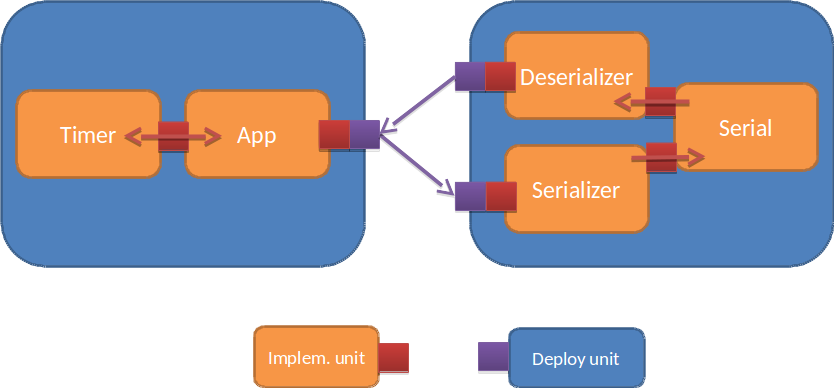
\includegraphics[width=0.8\linewidth]{figures/fig2}
	\caption[Heads implementation and deploy units integration]{Heads implementation and deploy units integration}
	\label{fig:fig2}
\end{figure}

Once wrapped into deploy units, components can be manipulated by the HEADS Deployment Language and actually deployed on the HEADS runtime platform, which evolves the Kevoree platform~\cite{DBLP:conf/cbse/FouquetMFBPJ12} initially developed for Java in order to also support JavaScript and more recently, .NET. The HEADS Deployment Language provide a way to write scripts describing which components to instantiate, how to configure them (set values of parameters), and how to connect components through communication channels. A large set of components and channels is already available off the shelf. At deployment time, the script, describing the components and channels deployed on the different nodes of the system, will be sent to the different nodes, which will interpret this script and actually deploy the necessary components, etc.   

The HEADS Deployment Language and Runtime platforms are available as a set of open-source projects on GitHub\footnote{https://github.com/dukeboard/kevoree\\https://github.com/kevoree/kevoree-js}.
